%------------------------------------------------

\begin{fullwidth}
Publication of any research product typically involves many iterations of
data, code, and code output files, with inputs from multiple collaborators.
This process can quickly become unwieldy.
It is in nobody's interest for a skilled and busy researcher
to spend days re-numbering figures, tables, or references (and it can take days)
when a reasonable amount of up-front effort can automate the task.
Similarly, simultaneous collaboration should not involve
the repetitive and error-prone task of manually resolving
sets of tracked-changes documents with conflicting edits.
Furthermore, for most development data projects,
completing a research output is not the end of the task.
Academic journals and policy notes are more commonly supported by
reproducibility packages which contain the data, code, and supporting materials
needed to recreate the results.
Preparation of a reproducibility package is a pre-requisite
to formal publication at DIME,
and extensive reproducibility packages are now required at many major academic outlets.
Replication materials represent an intellectual contribution in their own right,
because they enable others to learn from your process
and better understand the results you have obtained.

In this chapter, we suggest tools and workflows for
efficiently managing collaboration on research and policy outputs
and ensuring reproducibility of their results.
First, we discuss how to use dynamic documents to collaborate on writing.
Second, we provide guidelines for preparing
functioning and informative reproducibility packages.
If you have organized your analysis process
according to the general principles outlined in earlier chapters,
preparing to publish materials will not require
substantial reorganization of the work you have already done.
Hence, publication is the conclusion of the system
of transparent, reproducible, and credible research we introduced
from the very first chapter of this book.
We include specific guidance on publishing both code and data files,
noting that these can be a significant contribution in addition to written results.
In all cases, we note that technology is rapidly evolving
and that specific tools noted here may not remain cutting-edge,
but the core principles involved in publication and transparency will endure.
\end{fullwidth}

%------------------------------------------------

\section{Preparing written documents for publication}

% collaborating is easier with dynamic documents
Development research is increasingly a collaborative effort.
This reflects changes in the economics discipline overall:
the number of sole-authored research outputs is decreasing,
and the majority of recent papers in top journals have three or more
authors.\cite{kuldtrend}
As a consequence, documents typically pass back and forth between several writers
before they are ready for publication or release.
As in all other stages of the research process,
effective collaboration requires the adoption of tools and practices
that enable version control and simultaneous contributions.
This book, for example, was written in {\LaTeX} and managed on GitHub.\sidenote{\url{
		https://github.com/worldbank/dime-data-handbook}}
As we outlined in the previous chapter,
\textbf{dynamic documents} are a way to simplify writing workflows:
updates to code outputs that appear in these documents, such as tables and figures,
can be passed in to the final research output in a single click,
rather than copy-and-pasted or otherwise handled individually.
Managing the writing process in this way
improves organization and reduces error,
such that there is no risk of materials being compiled
with out-of-date results, or of completed work being lost or redundant.

\subsection{Preparing formal outputs as {\LaTeX} documents}

\begin{fullwidth}
	\begin{figure}
		\centering
		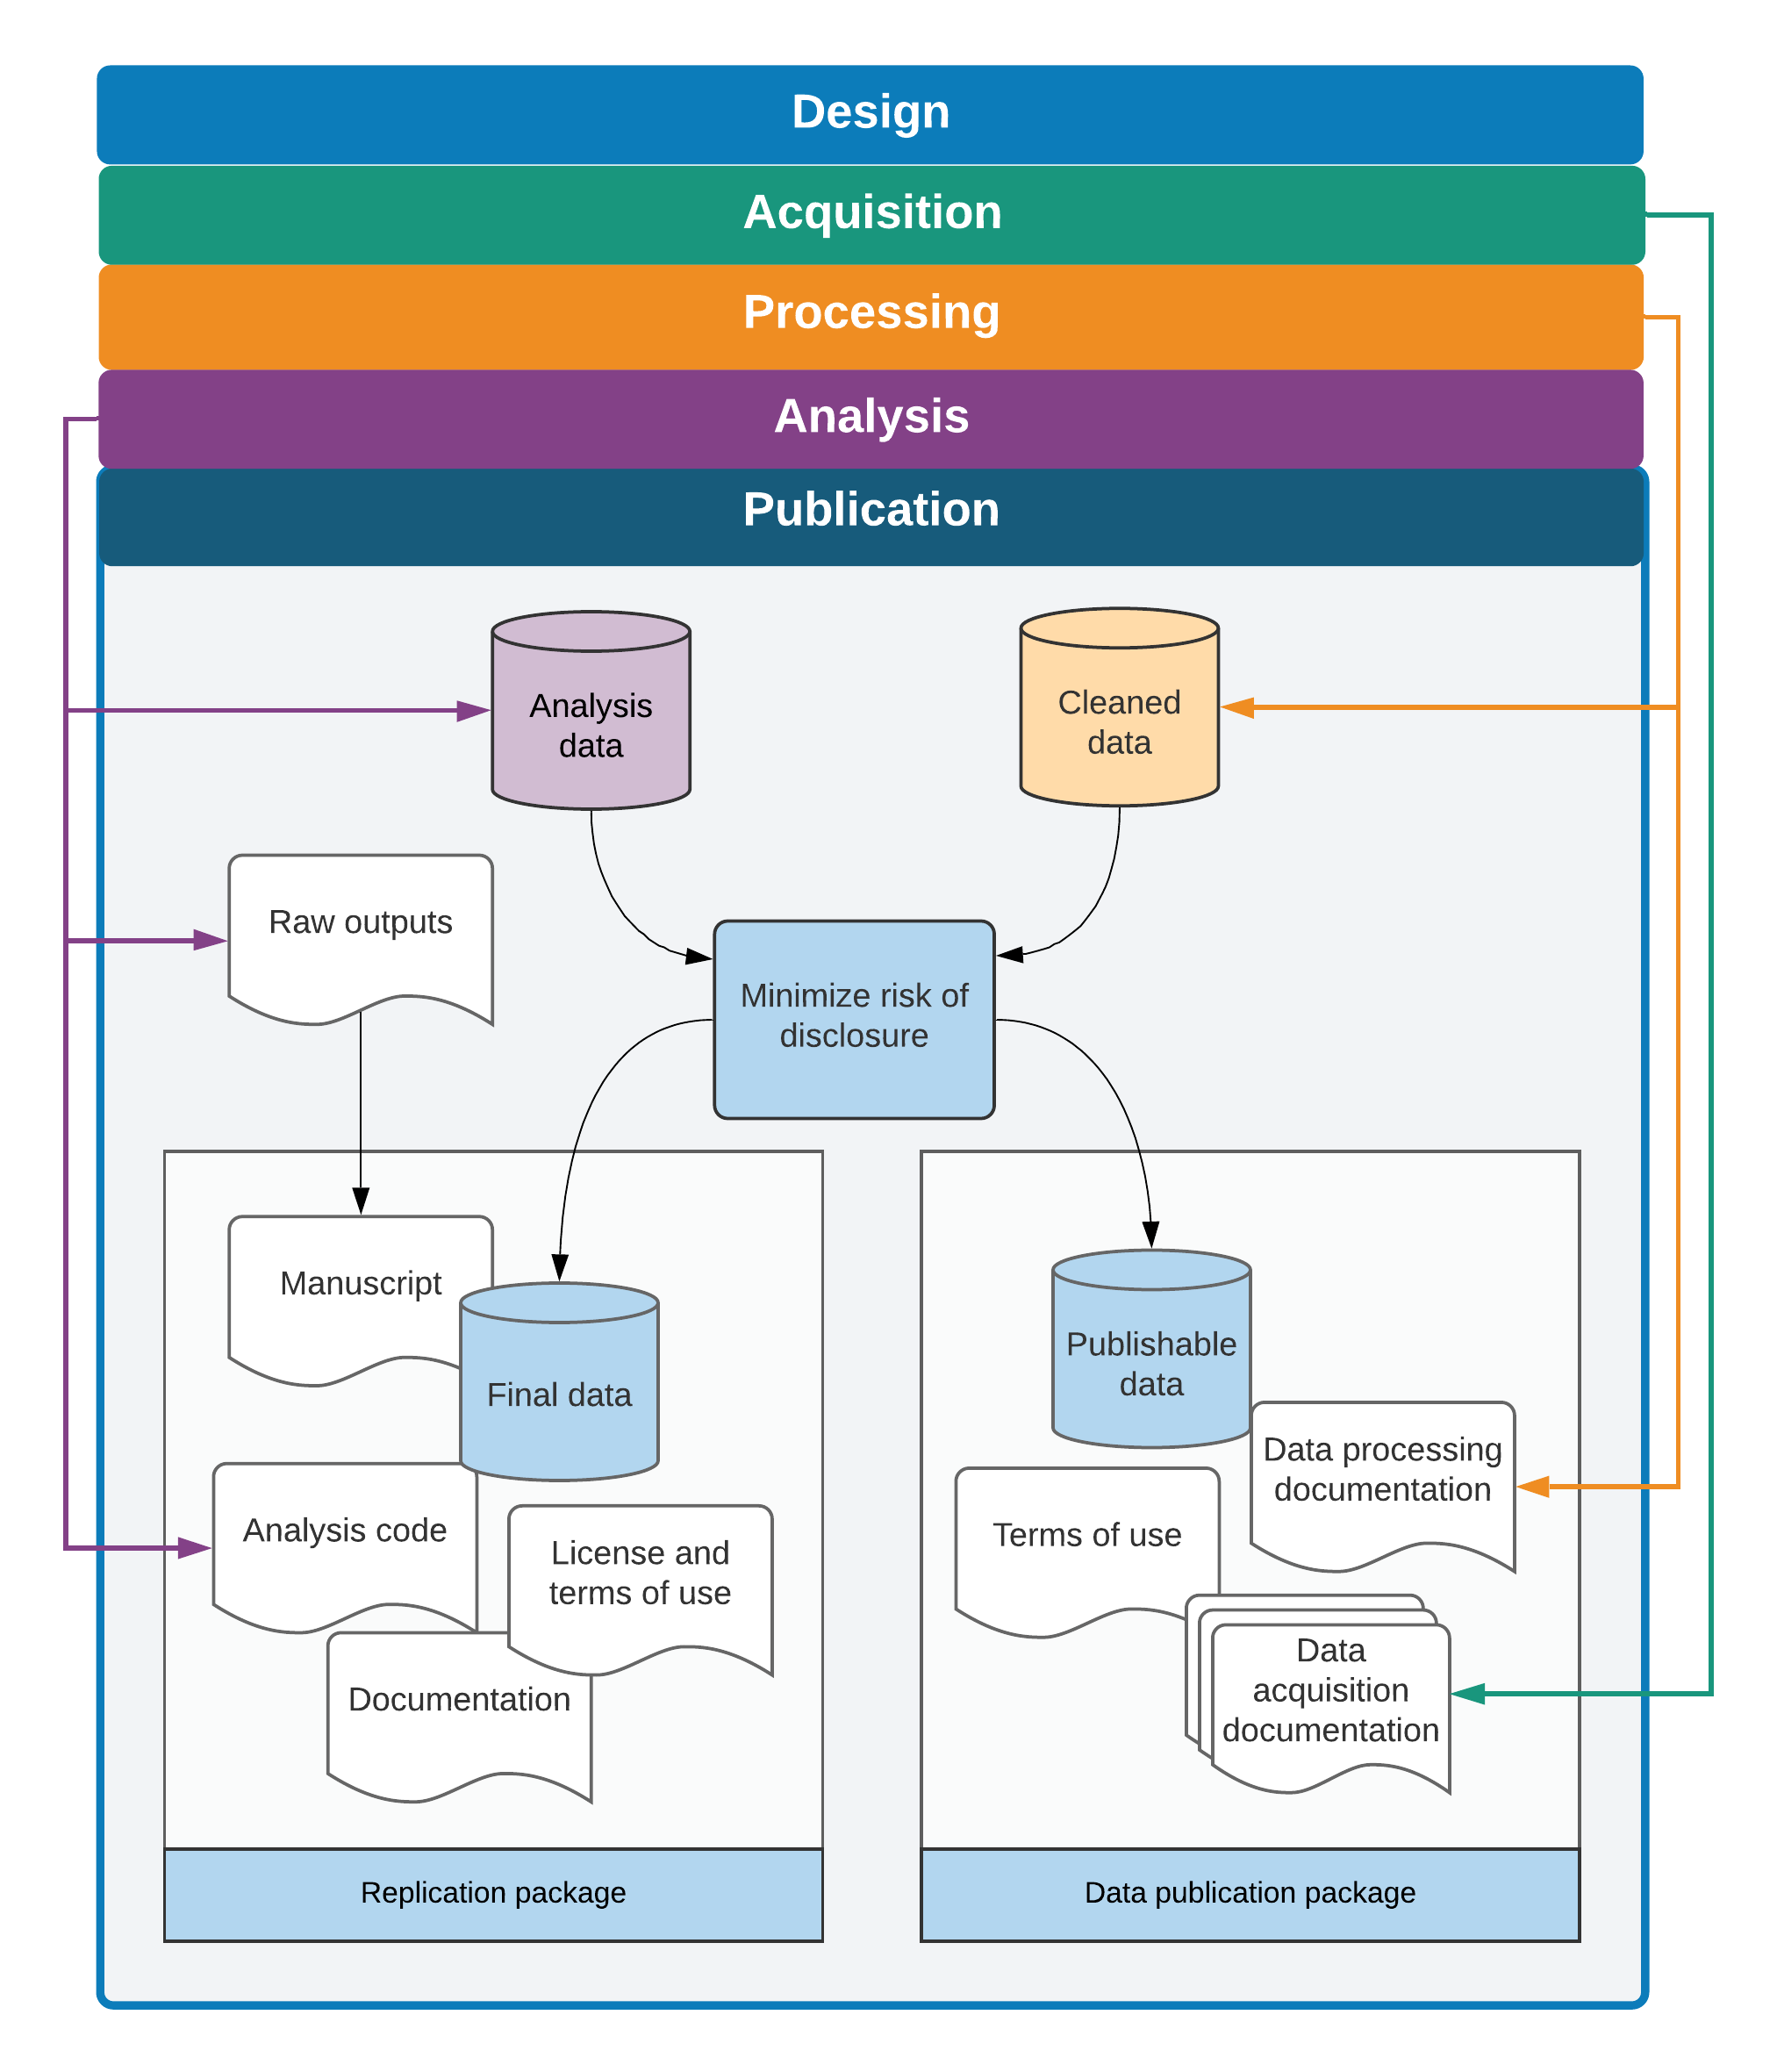
\includegraphics[width=1.6\linewidth]{diagrams/Publication}
		\caption{}
		\label{fig:intro}
	\end{figure}
\end{fullwidth}

% what exactly is a dynamic document
As we discussed in Chapter 6, the most widely used software
for dynamically managing formal manuscripts and policy outputs is {\LaTeX}.
It is also becoming more popular for shorter documents,
such as policy briefs,
with the proliferation of skills and templates for these kinds of products.
\index{\LaTeX}
{\LaTeX} uses explicit references to the file path of each input (e.g. tables and figures),
which are reloaded from these locations every time the final document is compiled.
This is not possible by default in, for example, Microsoft Word.
There, you have to copy and paste each object
whenever tables, graphs, or other inputs are updated.
As time goes on, it becomes increasingly likely
that a mistake will be made or something will be missed.
In {\LaTeX}, instead of writing in a
``what-you-see-is-what-you-get'' mode as you do in Word,
you write plain text in a \texttt{.tex} file,
interlaced with coded instructions formatting the document and linking to exhibits (similar to HTML).
{\LaTeX} manages tables and figures dynamically
and includes commands for simple markup
like font styles, paragraph formatting, section headers and the like.
It includes special controls for
footnotes and endnotes, mathematical notation, and bibliography preparation.
It also allows publishers to apply global styles and templates to already-written material,
reformatting entire documents in house styles with only a few keystrokes.

% keeping it simple
To create a {\LaTeX} document,
you will typically start from a new top-level directory for each research output.
For a single output, we recommend putting the core document files
(such as \texttt{main.tex} and \texttt{bibliography.bib})
in the top-level folder,
and then have subfolders for figures, tables, and other inputs.
Your analysis scripts should be set up such that it is easy to output files
at the location of your choice by adjusting paths in the master script.
Above all, keep your workflow as simple as possible.
While {\LaTeX} \textit{can} produce complex formatting,
this is rarely needed for academic publishing,
as academic manuscripts will usually be reformatted
based on the style of the publisher.
(By contrast, policy and other self-produced documents may desire
extensive typesetting and investments in custom templates and formatting.)
So, in academia at least,
it's rarely worth the investment to go beyond basic {\LaTeX} tools:
the title page, sections and subsections,
figures and tables, mathematical equations,
bolding and italics, footnotes and endnotes,
and, last but not least, references and citations.

% managing references in LaTeX
One of the most important tools available in {\LaTeX}
is the BibTeX citation and bibliography manager.\cite{kopka1995guide}
BibTeX keeps all the references you might use in an auxiliary \texttt{.bib} file,
then references them using a simple command typed directly in the document.
Specifically, {\LaTeX} inserts references in text using the \texttt{\textbackslash cite\{\}} command.
Once this is written, {\LaTeX} automatically pulls all the citations into text
and creates a complete bibliography based on the citations you used whenever you compile the document.
The system allows you to specify exactly how references should be displayed in text
(such as superscripts, inline references, etc.)
as well as how the bibliography should be styled and in what order
(such as Chicago, MLA, Harvard, or other common styles).
The same principles that apply to figures and tables are therefore applied here:
You can make changes to the references in one place (the \texttt{.bib} file),
and then everywhere they are used they are updated correctly with one process.
BibTeX is so widely used that it is natively integrated in Google Scholar.
To obtain a reference in the \texttt{.bib} format for any paper you find,
click ``BibTeX'' at the bottom of the Cite window (below the preformatted options).
Then, copy the code directly into your \texttt{.bib} file.
They will look like the following:

\codeexample{sample.bib}{./code/sample.bib}

\noindent BibTeX citations are then used as follows:

\codeexample{citation.tex}{./code/citation.tex}

With this tool, you can ensure that references are handled
in a format you can manage and control.\cite{flom2005latex}
By changing some settings in the document itself,
you can change the style of inline citations and bibliographical references.
You can, for example, use superscripts or author names inline,
and order the bibiliography either by order of appearance or alphabetically.
All the formatting and numbering will be handled automatically.
You can also choose to display only the references which are cited in the text,
or to include every reference in the \texttt{.bib} file.
Since different publishers have different requirements,
it is quite useful to be able to adapt this and other formatting very quickly,
including through using publisher-supplied templates where available.

% using pandoc to convert LaTeX into word
Because it follows a standard code format,
{\LaTeX} has one more useful trick:
you can convert the raw document into Word
or a number of other formats
using utilities such as \texttt{pandoc}.\sidenote{\url{https://pandoc.org}}
Even though conversion to Word is required
for a number of academic publishers and can even be preferred for some policy outputs,
we still recommend using {\LaTeX} to prepare these when possible.
You should export to Word only at the final stage, when submitting materials.
You can also use a CSL (Citation Styles Library) file\sidenote{
  \url{https://github.com/citation-style-language/styles}}
for nearly any journal and have it applied automatically in this process.
Therefore, even in the case where you are required to provide
\texttt{.docx} versions of materials to others, or tracked-changes versions,
you can create them effortlessly from a {\LaTeX} document,
then use external tools like Word's compare feature
to generate integrated track-changes versions when needed.

\subsection{Getting started with {\LaTeX} as a team}

Getting used to {\LaTeX} can be challenging,
but the control it offers over the writing process is invaluable.
Because it is written in a plain text file format,
\texttt{.tex} can be version-controlled using Git.
This makes it possible to manage contributions and version histories
using the same system we recommend for data work.
DIME Analytics has created a variety of templates and resources
that you can adapt for your own team.\sidenote{
	\url{https://github.com/worldbank/DIME-LaTeX-Templates}}
Integrated editing and compiling tools like TeXStudio\sidenote{
  \url{https://www.texstudio.org}}
and \texttt{atom-latex}\sidenote{
  \url{https://atom.io/packages/atom-latex}}
offer the most flexibility to work with {\LaTeX} in teams.

% cloud-based implementations are a good place to start
Although ultimately worth it, setting up {\LaTeX} is not always simple,
particularly if you are new to working with plain text code and file management.
This is because {\LaTeX} requires that all formatting be done in its special code language,
and it is not always informative when you do something wrong.
This can be off-putting very quickly for people
who simply want to get to writing,
and staff not used to programming may not easily acquire the necessary knowledge.

Cloud-based implementations of {\LaTeX} can make it easier for your team to use
{\LaTeX} without all members having to invest in new skills,
and can be particularly useful for first forays into {\LaTeX} writing.
One example of this is Overleaf.\sidenote{
  \url{https://www.overleaf.com/}}
Most such sites offer a subscription feature
with useful extensions and various sharing permissions,
and some offer free-to-use versions with basic tools that are sufficient
for a broad variety of applications,
up to and including writing a complete academic paper with coauthors.

% Advantages of cloud-based implementations
Cloud-based implementations of {\LaTeX} have several advantageous features
for teams compared to classic desktop installations.
First, since they are completely hosted online,
they avoid the inevitable troubleshooting required to set up a {\LaTeX} installation
on various personal computers run by the different members of a team.
Second, they typically maintain a single, continuously synced, master copy of the document
so that different writers do not create conflicted or out-of-sync copies,
or need to deal with Git themselves to maintain that sync.
Third, they typically allow collaborators to edit documents simultaneously,
though different services vary the number of collaborators and documents allowed at each tier.
Fourth, some implementations provide a ``rich text'' editor
that behaves pretty similarly to familiar tools like Word,
so that collaborators can write text directly into the document without worrying too much
about the underlying {\LaTeX} coding.
Cloud services also usually offer a convenient selection of templates
so it is easy to start up a project and see results right away
without needing to know a lot of the code that controls document formatting.

% Disadvantages of cloud-based implementations
Cloud-based implementations of {\LaTeX} also have disadvantages.
There is still some up-front learning required, unless you're using the rich text editor.
Continuous access to the internet is necessary,
and updating figures and tables requires a bulk file upload that is tough to automate.
They vary dramatically in their ability to integrate
with file systems where you store your code and code outputs,
and so you will need to practice an integrated workflow depending what is available to you.
Some teams adopt cloud-based tools as a permanent solution,
though our recommendation is to eventually shift to
local editing and compiling using tools such as TexStudio and code editors like Atom.

%----------------------------------------------------

\section{Preparing and publishing data}

% what are reproducibility packages and what they must contain
While we have focused so far on written materials,
you must also consider how you will publish
the data used in your research.
The open science community at large sees data publication
both as a citable output and as a necessary transparency measure.
Fortunately, it is a conceptually simple task to produce
and catalog the required materials.
You should be prepared to catalog two separate collections.
First, you should catalog the unaltered (de-identified) data
with all variables corresponding directly
to fields in the original dataset or data collection instrument
(this may not be necessary if you are working with secondary data that is published elsewhere in this format).
If you follow the steps outlined in Chapter 5,
when you get to the publication stage you will have
a cleaned data set and supporting documentation ready.
Second, you should separately catalog
the analysis dataset used for the research output you are publishing.
This is typically included in the replication package.
The package should also include the data construction scripts
that create transformed and derived indicators,
project-specific information
such as treatment assignment and other indicators
generated directly by the research team (another example is constructed record linkages).
If you followed the workflow recommended in Chapter 6,
by the time you reach publication stage you will already have all necessary
files and documentation at hand.

\subsection{De-identifying data for publication}

% what is final de identification
Before publishing data,
you should carefully perform a \textbf{final de-identification}.
The objective of de-identification is to reduce the risk of disclosing confidential information in the published dataset.
If you are following the workflow outlined in this book,
you should have already removed direct identifiers as a first step after acquiring the data
(see the discussion of initial de-identification in Chapter 5).
For the final de-identification, you should additionally remove
indirect identifiers, and assess the statistical disclosure risk of your data.\sidenote{
	\textbf{Disclosure risk:} the likelihood that a released data record can be associated with an individual or organization.}\index{statistical disclosure}
Unlike direct identifiers, for which a link (or lack thereof) to public information is verifiable,
indirect identifiers require an assessment of the likelihood
that an individual can be singled out in the data
and then linked to public information using combinations of available data.
For example, seemingly innocuous variables such as US zip code,
gender, and date of birth uniquely identify
approximately 87\% of the US population.\cite{Sweeney2000}.
In development data, information such as the size of a household,
the ages and marital statuses of the household members,
and the types of work or schooling they engage in
may be more than enough to identify a person or family
from a sufficiently small group.

% tools for final de-identification: pii_detection, pii-scan, sdcMicro
A number of tools have been developed to help researchers de-identify data.
At this stage, the World Bank's \texttt{sdcMicro} tool,\sidenote{
	\url{https://sdcpractice.readthedocs.io}}
has a useful feature
that allows you to assess the uniqueness of the records in your data.
It produces simple measures of the identifiability of records from
the combination of potentially indirectly identifying variables,
and allows you to apply common information masking algorithms,
such as binning, top-coding, and jittering data prior to release.
You should determine how sensitive your results are to these transformations;
it may be the case that this data cannot be used for your reproducibility package.

% trade-off between accuracy and privacy
There will almost always be a trade-off between accuracy and privacy.
For publicly disclosed data, you should favor privacy.
Stripping identifying variables from a dataset may not be sufficient to protect respondent privacy,
due to the risk of re-identification.
One solution is to add noise to data, as the US Census Bureau has proposed.\cite{abowd2018us}
This makes the trade-off between data accuracy and privacy explicit.
But there are not, as of yet, established norms for such ``differential privacy'' approaches:
most approaches fundamentally rely on judging ``how harmful'' information disclosure would be.
The fact remains that there is always a balance between information release (and therefore transparency)
and privacy protection, and that you should engage with it actively and explicitly.
The best thing you can do is make a complete record of the steps that have been taken
so that the process can be reviewed, revised, and updated as necessary.

Removing variables results in loss of information, so the de-identification process
requires careful assessment of the potential risk to the individual
that could be caused by disclosure of their identity or personal information.
This will vary widely depending on the types of information
you are collecting and the overall vulnerability of the population.
In extreme cases, where the population is highly vulnerable
and combinations of information are highly specific,
you may not be able to publicly release any data at all.
You will still be expected to catalog and cite your data,
even if you cannot release it publicly.
In practice, this may mean publishing only a catalog entry
providing information about the contents of the datasets
and how future users might request permission to access them
(even if you are not the person to grant that permission).
In some cases, it may be possible to release the dataset but
embargoing specific variables that are required for the analysis but cannot be released publicly.
It may be necessary to grant access to the embargoed data for specific purposes,
such as a computational reproducibility check required for publication,
if done under careful data security protocols and approved by an IRB.

\subsection{Publishing raw and constructed datasets}

% options for when the data cannot be published
Publicly documenting all original data acquired as part of a research project
is an important contribution in its own right.
Cataloging and/or archiving original datasets
is a significant contribution in addition to any publication of analysis results.\sidenote{
	\url{https://dimewiki.worldbank.org/wiki/Publishing_Data}}
Publicly releasing data allows other researchers
to validate the mechanical construction of your results,
investigate what other results might be obtained from the same population,
and test alternative approaches or answer other questions.
This fosters collaboration and may enable researchers to explore variables and
questions that you do not have time to focus on otherwise.

% platforms for publishing data
The first step toward data publication is choosing the platform where you will publish your data.
A variety of options exist;
it is important to choose one that allows you to obtain a digital object identifier (DOI)
for the location of your data (even if its URL changes),
and a formal citation for your data, so you can reference it in other research outputs.\sidenote{url{https://www.doi.org}}
Two common platforms for development data are the World Bank's Development Data Hub
and Harvard University's Dataverse.
The World Bank's Development Data Hub\sidenote{
	\url{https://datacatalog.worldbank.org}}
includes a Microdata Catalog\sidenote{
  \url{https://microdata.worldbank.org}}
and a Geospatial Catalog,
where researchers can publish data and documentation for their projects.\sidenote{
  \url{https://dimewiki.worldbank.org/Microdata\_Catalog}
\newline
  \url{https://dimewiki.worldbank.org/Checklist:\_Microdata\_Catalog\_submission}}
The Harvard Dataverse publishes both data and code,
and its repository
Datahub for Field Experiments in Economics and Public Policy\sidenote{
	\url{https://dataverse.harvard.edu} and
	\url{https://dataverse.harvard.edu/dataverse/DFEEP}}
is especially relevant for impact evaluations.
Both the World Bank Microdata Catalog and the Harvard Dataverse
create data citations for deposited entries.
DIME has its own collection of datasets in the Microdata Catalog,
where data from our projects is published.\sidenote{\url{
		https://microdata.worldbank.org/catalog/dime}}

% check what you can and cannot publish
Once you have chosen a platform, you need to determine exactly what data you will publish.
As mentioned earlier, there are typically two different types of data releases for a research project:
complete (de-identified) original datasets and derivative datasets used for specific research outputs.
Whether you can publish the original dataset depends on data ownership and licensing agreements.
If the data was acquired through a survey that was contracted by the research team,
the data belongs to the research team,
and therefore the team has full publication rights for both the original and derivative data.
If data was acquired from a partner through a licensing agreement,
the terms of the license will determine publication rights.
These datasets should match the survey instrument or source documentation as closely as possible,
and should not include indicators constructed by the research team.
Even if you do not have rights to publish the original data,
you can typically publish derivative datasets prepared by the research team.
These datasets usually contain only the constructed indicators and associated documentation,\sidenote{
  \url{https://guide-for-data-archivists.readthedocs.io}}
and should also be included in the replication package.

% licensing published data
When publishing data,
you will decide how the data may be used and what license you will assign to it.\sidenote{
  \url{https://dimewiki.worldbank.org/Publishing_Data}}
Make sure you understand the rights associated with any data release
and communicate them to its future users.
Material without a license may never be reused.
You should prefer to offer a license that is explicit
and details whether and how specific individuals may access the data.
Terms of use available in the World Bank Microdata Catalog include,
in order of increasing restrictiveness:
\textit{open access}, \textit{direct access}, and \textit{licensed access}.\sidenote{
  \url{https://microdata.worldbank.org/index.php/terms-of-use}}
\textit{Open access} data is freely available to anyone, and simply requires attribution.
\textit{Direct access} data is available to registered users who agree
to use the data for statistical and scientific research purposes only,
to cite the data appropriately,
and not to attempt to identify respondents or data providers
or link the data to other datasets that could allow for re-identification.
\textit{Licensed access} data is restricted to bona fide users,
who submit a documented application detailing
how they will use the data and then sign a formal agreement governing data use.
The user must be acting on behalf of an organization,
which will be held responsible in the case of any misconduct.

% content of data publication: data files, meta data and dcumentation
Published data should be released in a widely recognized format.
While software-specific datasets are acceptable accompaniments to the code
(since those precise materials are probably necessary),
you should also consider releasing datasets in plain text formats
such as CSV files with accompanying codebooks,
since these can be used by any researcher.
Additionally, you should also release PDF or code versions of
the data collection instrument or survey questionnaire
so that readers can understand which data components are
collected directly in the field and which are derived.
With your analysis dataset,
you should also release the code
that constructs any derived measures
from the raw dataset,
so that others can learn from your work and adapt it as they like.

\section{Preparing a complete reproducibility package}

Major journals now often require that you provide both the data and code required to recreate your results.
Some even require being able to reproduce the results themselves
before they will approve a paper for publication.\cite{vilhuber2020report}
This set of materials, taken together,
is often referred to as a \textbf{reproducibility package}.
If you have followed the workflows described in this book,
preparing the replication package will only require a small amount of extra work.
If not, creating this package may take some time.
When the replication package is completed,
whoever downloads it should be able
to understand how your code produces results from your data
and be able to reproduce them exactly by executing the included master script.

\subsection{Organizing code for reproducibility}

% published code must be understandable
Before releasing your code, you should edit it for content and clarity
just as if it were written material.
The purpose of releasing code is to allow others to understand
exactly what you have done in order to obtain your results,
and enable them to apply similar methods in future projects.
Other researchers should be able to reproduce individual portions of your analysis
by making only small adjustments to your code.
In either a scripts folder or in the root directory,
you should include a master script that allows someone else to run the entire project
and re-create all raw code outputs by changing only a single line of code:
the one setting the directory path.
The code should both be functional and readable,
through the use of a clear structure and extensive commenting.
Code is often not written this way when it is first prepared,
so it is important for you to review the content and organization
so that a new reader can figure out what your code should do and how it does it.
Making code clean and readable is often where you need to invest time prior to releasing your reproducibility package.

% reproducibility review
DIME requires all academic outputs to successfully pass a computational reproducibility check
before being submitted for publication.
We have adopted several practices and requirements to support the production
of high-quality reproducibility packages.
The materials for these practices are publicly available,
so you can use them to check the reproducibility of your own work.
This reproducibility check is initiated by submitting the Reproducibility Package Checklist.\sidenote{
	\url{https://github.com/worldbank/dime-standards}}
DIME projects are required to organize code
with a master script, to facilitate handovers across team members
and make the computational reproducibility check a one-click exercise.
Compliance with these and other coding standards at DIME is monitored through
quarterly peer code review rounds, which allows research assistants to improve their code and documentation as it is written,
rather than revisiting it in a rush near publication time.
DIME projects are also expected to use Git and GitHub
to document project work and collaboration,
and to keep the master branch up-to-date as a working edition.\sidenote{
	\url{https://github.com/worldbank/dime-standards}}

% ensuring code reproducibility
Before publicly releasing a reproducibility package,
it is essential to make sure that the code runs identically
on your individual setup compared to
a fresh installation of your software.

To ensure that your code will run completely on a new computer,
you must install any required user-written commands in the master script
(for example, in Stata using \texttt{ssc install} or \texttt{net install}
and in R adding code that gives users the option to install packages,
including selecting a specific version of the package if necessary).
In many cases you can even directly provide the underlying code
for any user-installed packages that are needed to ensure forward-compatibility.
Make sure system settings like software version and memory settings are defined.
The \texttt{ieboilstart} command in \texttt{ietoolkit} defines and applies these settings
for a chosen Stata version.\sidenote{\url{https://dimewiki.worldbank.org/ieboilstart}}

% tracking code and outputs
Finally, make sure that code inputs and outputs are clearly identified.
A new user should, for example, be able to easily find and quickly recreate
any files generated by the code.
Readers should also be able to easily map all the outputs of the code
to where they appear in the associated published material,
so you must ensure ensure that the raw components of figures or tables are clearly identified.
Documentation in the master script is often used to indicate this information.
For example, code outputs should clearly correspond by name to an exhibit in the paper, and vice versa.
(Supplying a compiling {\LaTeX} document can support this.)
Code and code outputs which are not used in the final paper should be removed from the final replication package,
but still archived for transparency.
One way to do this is keeping them on a separate GitHub branch

\subsection{Releasing a reproducibility package}

% finding a place to publish the package
Once your replication package is prepared for public release,
you need to find a place to publish your materials.
At the time of writing, there is no consensus on the best solution for publishing code,
and there are a variety of archives and storage providers
that cater to different needs.
The technologies available are likely to change dramatically
over the next few years;
the specific solutions we mention here highlight some current approaches
as well as their strengths and weaknesses.

% code licenses
Features to look for in a platform to release reproducibility packages include:
the possibility to store data and documentation as well as code,
the creation of a static copy of its content, that cannot be changed or removed,
and the assignment of a permanent digital object identifier (DOI) link.
Unlike data, code usually has few external constraints to publication.
The research team owns the code in almost all cases,
and code is unlikely to contain identifying information
(though you must carefully verify that it does not).
Publishing code also requires assigning a license to it;
most code publishers offer extremely permissive licensing options by default (GitHub is a good example).
Note that if you do not provide a license, no one can use your code.
It is common to only require attribution and citation for code reuse,
without putting any barriers or restrictions to accessing the code.

% pros and cons of GitHub
One option for releasing a reproducibility package is GitHub.
Making a public GitHub is completely free.
It can hold any file types,
provide a structured, compressed download of your whole project,
and allow others to look at alternate versions or histories easily.
It is straightforward to simply upload a fixed directory to GitHub,
apply a sharing license, and obtain a URL for the whole package.
There is a strict size restriction of 100MB per file and
a restriction of 100GB on the size of the repository as a whole,
so larger projects will need alternative solutions.
However, GitHub is not the ideal platform on which to release reproducibility packages.
It is built to version control code, and to facilitate collaboration on it.
It is not an archive, meaning that it does not guarantee the permanence
of uploaded materials or the access URL,
and it does not manage citations or non-code licenses by default.
One suggestion is to combine GitHub with the Open Science Framework,\sidenote{
  \url{https://osf.io}}
as OSF can easily link to and import material from GitHub and
apply a permanent URL, DOI, formal citation, general license, and archival services to it.

% Other options: data verse, osf, research gate. what to look for before deciding
Other options include the Harvard Dataverse\sidenote{
  \url{https://dataverse.harvard.edu}}
and ResearchGate.\sidenote{
  \url{https://www.researchgate.net}}
Any of these archival services is acceptable --
the main requirement is that the system can handle
the structured directory that you are submitting,
and that it can provide a stable, URL for your project
and report exactly what, if any,
modifications you have made since initial publication.
You can even combine more than one tool if you prefer,
as long as they clearly reference each other.
For example, one could publish code and the corresponding license on GitHub
and point to data published on the World Bank Microdata Catalog.
Emerging technologies such as the ``containerization'' approach of CodeOcean\sidenote{
  \url{https://codeocean.com}}
offer to store both code and data in one repository,
and also provide an online workspace in which others can execute and modify your code
without having to download your tools and match your local environment.
This is particularly useful over time, as packages and other underlying software may have changed since publication.

% pre-prints
In addition to code and data,
you may also want to release an author's copy or preprint
of the article itself along with these raw materials.
Check with your publisher before doing so;
not all journals will accept material that has been publicly released
before its formal publication date, although,
in most development research fields,
the release of working papers is a fairly common practice.
This can be done on a number of preprint websites,
many of which are topic-specific.\sidenote{
  \url{https://arxiv.org/}}
You can also use GitHub or OSF and link to the PDF file directly
through your personal website or whatever medium you are sharing the preprint.
We recommend against using file sharing services such as
Dropbox or Google Drive for this purpose,
as their access is more restrictive,
and organizations limit access to platforms other than the one officially adopted.
